\documentclass[xcolor=dvipsnames]{beamer}
\usepackage{tikz,subcaption,amsmath,physics,xfrac,siunitx}
\usepackage{tikz-feynman}
\usetikzlibrary{shadings}
\setbeamercovered{highly dynamic}
% \tikzfeynmanset{compat=1.1.0}
\usetikzlibrary{shapes,arrows,decorations.pathmorphing,arrows.meta}


\tikzstyle{startstop} = [rectangle, rounded corners, minimum width=3cm, minimum height=1cm,text centered, draw=black]
\tikzstyle{io} = [trapezium, trapezium left angle=70, trapezium right angle=110, minimum width=3cm, minimum height=1cm, text centered, draw=black]
\tikzstyle{process} = [rectangle, minimum width=3cm, minimum height=1cm, text centered, draw=black]
\tikzstyle{decision} = [diamond, minimum width=3cm, minimum height=1cm, text centered, draw=black]
\tikzstyle{arrowdiag} = [thick,->,>=stealth]

\usepackage{booktabs}
\usetheme{Madrid}
\useoutertheme[subsection=true,footline=authorinstitutetitle]{miniframes} % Alternatively: miniframes, infolines, split
\useinnertheme{circles}
\beamertemplatenavigationsymbolsempty

% \definecolor{PrimeCol}{RGB}{21,96,100} % UBC Blue (primary)
% \definecolor{SecCol}{RGB}{0,196,154} % UBC Grey (secondary)
% \definecolor{AlertCol}{RGB}{244,96,54}
% \definecolor{PrimeCol}{RGB}{26,50,96}
\definecolor{PrimeCol}{RGB}{11, 79, 108}
% \definecolor{SecCol}{RGB}{69,203,232}
\definecolor{SecCol}{RGB}{31, 122, 140}

\definecolor{ThirCol}{RGB}{192,199,119}
\definecolor{AlertCol}{RGB}{241,127,41}





\setbeamerfont{author}{size=\Large}
\setbeamerfont{institute}{size=\normalsize\itshape}
\setbeamerfont{title}{size=\fontsize{30}{36}\bfseries}
\setbeamerfont{subtitle}{size=\Large\normalfont\slshape}



\setbeamercolor{palette primary}{bg=ThirCol,fg=white}
\setbeamercolor{palette secondary}{bg=SecCol,fg=white}
\setbeamercolor{palette tertiary}{bg=PrimeCol,fg=white}
\setbeamercolor{palette quaternary}{bg=black,fg=white}

\setbeamercolor{block title}{bg=PrimeCol,fg=white}
\setbeamercolor{block body}{bg=SecCol!10,fg=black}

\setbeamercolor{structure}{fg=PrimeCol} % itemize, enumerate, etc
\setbeamercolor{section in toc}{fg=PrimeCol} % TOC sections
\setbeamercolor{alerted text}{fg=AlertCol}
% Override palette coloring with secondary
\setbeamercolor{subsection in head/foot}{bg=SecCol,fg=white}
\setbeamercolor{frametitle}{fg=PrimeCol,bg=white}


\setbeamertemplate{title page}{%
\begin{tikzpicture}[remember picture,overlay,>=stealth',photon/.style={decorate,decoration={snake,post length=1mm}}]
\fill[PrimeCol]
  ([yshift=15pt]current page.west) rectangle (current page.south east);
\node[anchor=east] 
  at ([yshift=-30pt]current page.north east) (author)
  {\Huge\usebeamerfont{author}\color{PrimeCol} Gonçalo Garcês S.R. Baptista};
\node[anchor=north east] at ([yshift=-35pt]current page.north east)
{\footnotesize\color{PrimeCol} Bsc. in Physics Engineering};
\node[anchor=north east] at ([yshift=-50pt,xshift=.2cm]current page.north east){\footnotesize\color{PrimeCol}
\begin{tabular}{ r r}
 President:& Prof. André Wemans\\ 
 Rapporteur:& Prof. Jorge Sampaio\\  
 Advisor:& Prof. Mauro Guerra\\
 Co-Advisor:& Prof. Jorge Machado\\
\end{tabular}
};


\node[anchor=north east] 
  at ([yshift=-100pt]current page.north east) (institute)
  {\Large\usebeamerfont{institute} \color{PrimeCol} NOVA School of Science and Technology};
\node at ([yshift=-90pt,xshift=40pt]current page.north west) {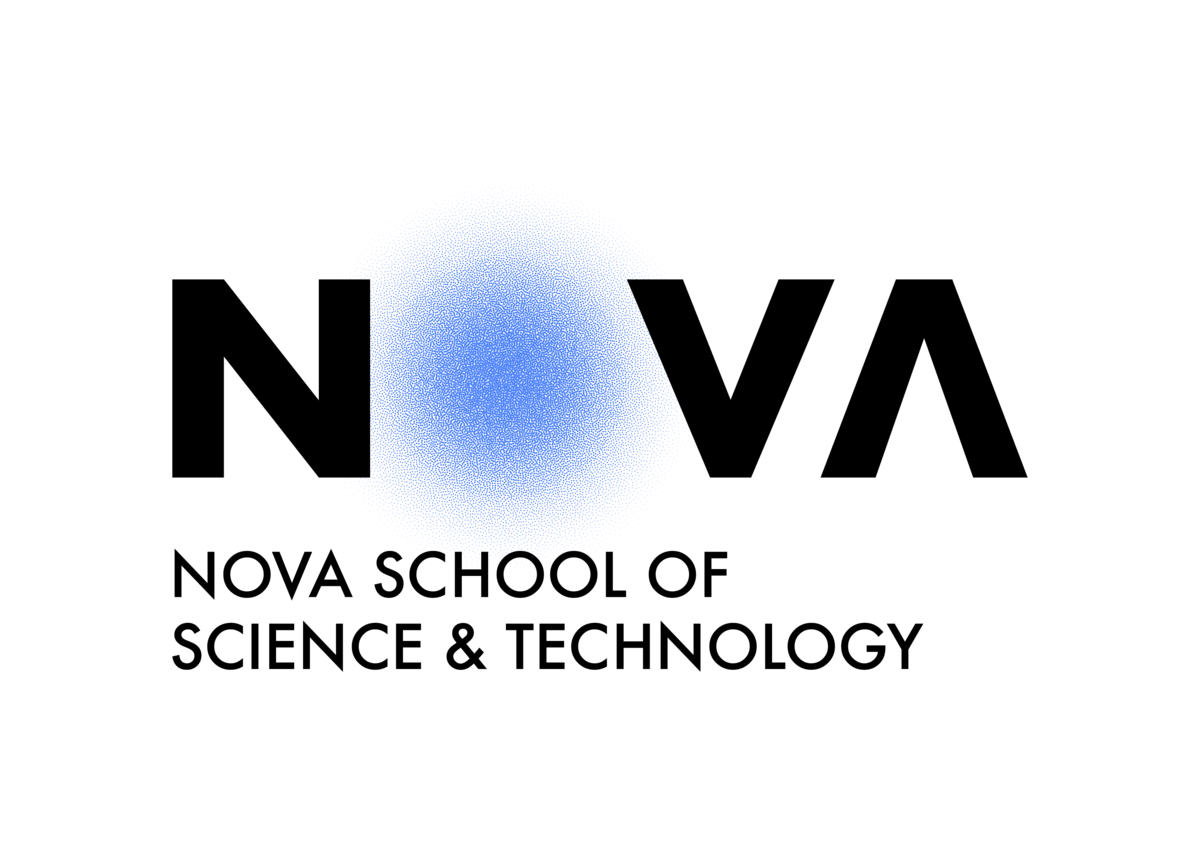
\includegraphics[width=3cm]{NovaLogo.png}};

\node at ([yshift=-30pt,xshift=30pt]current page.north west) {
\includegraphics[width=3.5cm]{logo_libphys.png}};




\node[anchor=east]
  at ([yshift=-10pt,xshift=-20pt]current page.east) (title)
  {\parbox[t]{.9\paperwidth}{\Large\color{white}X-ray Resonant Raman Scattering}};
\node[anchor=east]
  at ([yshift=-60pt,xshift=-20pt]current page.east) (subtitle)
  {\parbox[t]{.9\paperwidth}{\large\color{white} Spectra simulation from first principles\\for Copper below the ionization threshold\\ using high-performance computing}};

  \node at (current page.south east) [circle, draw, white, minimum size=10cm,dashed] {};
  
  \node at ([xshift=-3.54553390593cm,yshift=3.54553390593cm]current page.south east) [circle, draw,fill, white, minimum size=.5cm,opacity=.5] {};
  
  \node at (current page.south east) [circle, draw, white, minimum size=7.5cm,dashed]{} ;
  
  \node at ([xshift=-1.58481848cm,yshift=3.39865420cm]current page.south east) [circle, draw,fill, white, minimum size=.5cm,opacity=.5] {};
  
  \node at ([xshift=-0.3268340cm,yshift=3.735730cm]current page.south east) [circle, draw,fill, white, minimum size=.5cm,opacity=.5] {};
  
  \node at ([yshift=0.3268340cm,xshift=-3.735730cm]current page.south east) [circle, draw,fill, white, minimum size=.5cm,opacity=.5] {};
  
  \node at ([yshift=2.65165042945cm,xshift=-2.65165042945cm]current page.south east) [circle, draw,fill, white, minimum size=.5cm,opacity=.5] {};
  
  \node at ([yshift=1.58481848cm,xshift=-3.39865420cm]current page.south east) [circle, draw,fill, white, minimum size=.5cm,opacity=.5] {};
  
  \node at (current page.south east) [circle, draw, white, minimum size=5cm,dashed]{} ;
  
  \node at ([xshift=-2.5cm]current page.south east) [circle, draw,fill, white, minimum size=.5cm,opacity=.5] {};
  
  \node at ([yshift=2.5cm]current page.south east) [circle, draw,fill, white, minimum size=.5cm,opacity=.5] {};
  
  \node at ([xshift=-1.76777cm,yshift=1.76777cm]current page.south east) [circle, draw,fill, white, minimum size=.5cm,opacity=.5] {};
  
  \node at (current page.south east) [circle, draw, white, minimum size=2.5cm,dashed]{} ;
  
  \node at ([xshift=-0.8838835cm,yshift=0.8838835cm]current page.south east) [circle, draw,fill, white, minimum size=.5cm,opacity=.5] {};

  \draw[->,photon,white,opacity=.5] (current page.south east) -- node[below left] {} ([xshift=-5cm,yshift=5cm]current page.south east);

    \begin{feynman}
      % Specify your vertices using coordinates
      \vertex (a) at ([yshift=.3cm,xshift=3cm]current page.south west);
      \vertex [left =.375cm of a] (a1);
      \vertex [above =.75cm of a1] (a11);
      \vertex [left = .75cm of a1] (a2);
      \vertex [left = .75cm of a2] (a3);
      \vertex [right =.75cm of a] (b);
      \vertex [above =.75cm of b] (c);
      \vertex [above = .75cm of c] (d);
      \vertex [right = .75cm of b] (e);
      \vertex [right = .375cm of e] (f);
      \vertex [above = .75cm of f] (f1);
      \vertex [right = .75cm of f1] (f2);
      \vertex [right = .375cm of f2] (f3);
      \vertex [below = .75cm of f3] (f4);
      \vertex [right = .75cm of f4] (f5);
      % \vertex [right = .375cm of a] (point1);
      % \vertex [above = .375cm of point1] (point2);
      
      % Draw the Feynman diagram edges
      \diagram* {
        (a) -- [white,opacity=.5,half right,photon] (a2),
        (a2) -- [white,opacity=.5] (a3),
        (a) -- [white,opacity=.5] (b),
        (a) -- [white, opacity=.5] (a2),
        (b) -- [photon,white,opacity=.5] (c),
        (c) -- [fermion, half left,white,opacity=.5,looseness=1.8] (d),
        (d) -- [fermion, half left ,white,opacity=.5,looseness=1.8] (c),
        (b) -- [white, opacity=.5] (e),
        (e) -- [white, opacity=.5] (f),
        (e) -- [white, opacity=.5,quarter left,photon] (f1),
        (f1) -- [white, opacity=.5,half left,fermion,] (f2),
        (f2) -- [white, opacity=.5,half left,fermion] (f1),
        (f2) -- [white, opacity=.5,quarter left,photon] (f4),
        (f)  -- [white, opacity=.5] (f5),
      };
    \end{feynman};
  
\end{tikzpicture}
% \begin{tikzpicture}
%     \begin{feynman}
%     \vertex (i1) at (current page.south) ;
%     \vertex (f1) at (current page.south) ;
%     \diagram* {
%       i1[particle=$\ell$] --[fermion] f1 [particle=$i$]};
%   \end{feynman}
% \end{tikzpicture}
}



\author{Gonçalo Baptista}
\institute{NOVA School of Science and Technology}
\title{X-ray Resonant Raman Scattering}
\subtitle{an ab-initio calculation}



%%%%%%%%%%%%%%
\setbeamertemplate{bibliography item}{\insertbiblabel} %% Remove book symbol from references and add number
\usepackage[style=ieee,backend=bibtex,citetracker=true]{biblatex}
\addbibresource{bibliography.bib}










\newcommand<>{\uncovergraphics}[2][{}]{
    % Taken from: <https://tex.stackexchange.com/a/354033/95423>
    \begin{tikzpicture}
    \node[anchor=south west,inner sep=0] (B) at (4,0)
        {\includegraphics[#1]{#2}};
    \alt#3{}{%
        \fill [draw=none, fill=white, fill opacity=0.9] (B.north west) -- (B.north east) -- (B.south east) -- (B.south west) -- (B.north west) -- cycle;
    }
    \end{tikzpicture}
}



% \title[Title Without Rambling]{My Rambling Presentation Title}
% \date{\today}
% \author[G.B.]
% {Gonçalo Garcês Sobreira Rodrigues Baptista}
% \institute[NOVA-SST]{RamblingAcademic.com\\Nuts and Bolts of Research. Plus Some Rambling.}
\AtBeginSection[]
{
    \miniframesoff
 \begin{frame}<beamer>
 \frametitle{Overview}
    \begin{columns}[T]
        \begin{column}{.45\textwidth}
            \tableofcontents[currentsection,sections=1-2]
        \end{column}
        \begin{column}{.45\textwidth}
            \tableofcontents[currentsection,sections=3-]
        \end{column}
    \end{columns}
 \end{frame}
 \miniframeson
}

\makeatletter
\let\beamer@writeslidentry@miniframeson=\beamer@writeslidentry%
\def\beamer@writeslidentry@miniframesoff{%
  \expandafter\beamer@ifempty\expandafter{\beamer@framestartpage}{}% does not happen normally
  {%else
    % removed \addtocontents commands
    \clearpage\beamer@notesactions%
  }
}
\newcommand*{\miniframeson}{\let\beamer@writeslidentry=\beamer@writeslidentry@miniframeson}
\newcommand*{\miniframesoff}{\let\beamer@writeslidentry=\beamer@writeslidentry@miniframesoff}
\makeatother

\begin{document}
	
	\begin{frame}[plain]
		\titlepage
	\end{frame}
	

	
	\section{Theoretical Introduction}
    \subsection{Characteristic x-rays}
    \begin{frame}{X-ray applications}
        \begin{figure}[h!]
            \centering\hfill
            \begin{subfigure}{0.3\textwidth}
            \uncovergraphics<1->[width=\linewidth]
            {medical_xray.jpg}
            \uncover<1->{\caption{Imaging purposes}}
            \end{subfigure}
            \begin{subfigure}{0.33\textwidth}
            \uncovergraphics<2->[width=\linewidth]{500uL.pdf}
            \uncover<2->{\caption{Sample quantification}}
            \end{subfigure}\hfill
            \begin{subfigure}{0.33\textwidth}
            \uncovergraphics<3->[width=\linewidth]
            {KAlpha.pdf}
            \only<1-3>{\uncover<3->{\caption{Fundamental parameters}}}
            \only<4>{\caption{\alert{Fundamental parameters}}}
            \end{subfigure}\hfill
            \caption{Application examples of x-ray radiation}
        \end{figure}
    \end{frame}

\begin{frame}{Vacancy generation and relaxation processes}
\begin{columns}[T,onlytextwidth]
    \column{0.5\textwidth}
    \begin{center}\vspace{-1cm}
    \begin{tikzpicture}[>=stealth',photon/.style={decorate,decoration={snake,post length=1mm}}]
        \draw (0,0) -- (0,1);
        \draw (0,1.2) -- (0,5);
        \draw[-Stealth] (0,5.2) -- (0,6);
        \shade[bottom color=black, top color= white] (0.2,5.3) rectangle (4.2,6);
        
        \draw (-0.1,4.9) -- (0.1,5.1);
        \draw (-0.1,5.1) -- (0.1,5.3);
        \draw (-0.1,0.9) -- (0.1,1.1);
        \draw (-0.1,1.1) -- (0.1,1.3);
        \node[anchor=east,align=center] at (-0.1,0.5) {Inner\\shell};
        \node[anchor=east,align=center] at (-0.1,2.7) {Outer\\shells};
        \node[anchor=east] at (0,6) {$E$};
        
        \draw (0.2,0.5) -- (4.2,0.5);
        \draw (-0.1,0.5) -- (0.1,0.5);
        \draw (.2,2)   --  (4.2,2);
        \draw (.2,2.7)   --  (4.2,2.7);
        \draw(.2,4)  -- (4.2,4);

        
        \draw[fill=SecCol](0.2+4/3,0.5)circle (.2cm);
        \only<1,2,6->{\draw[fill=SecCol](0.2+8/3,0.5)circle (.2cm)};
        \draw[fill=SecCol](0.2+4/3,2)circle (.2cm);
        \only<1-5>{\draw[fill=SecCol](0.2+8/3,2)circle (.2cm)};
        \draw[fill=SecCol](0.2+4/3,2.7)circle (.2cm);
        \draw[fill=SecCol](0.2+8/3,2.7)circle (.2cm);
        \only<-6>{\draw[fill=SecCol](0.2+4/3,4)circle (.2cm)};
        \draw[fill=SecCol](0.2+8/3,4)circle (.2cm);

        \only<3,4,5>{\draw[fill=SecCol,opacity=.3,dashed](0.2+8/3,0.5)circle (.2cm)};
        \only<6->{\draw[fill=SecCol,opacity=.3,dashed](0.2+8/3,2)circle (.2cm)};
        \only<3,7>{\draw[fill=SecCol](0.2+6/3,6)circle (.2cm)};
        \only<7>{\draw[fill=SecCol,dashed,opacity=.3](0.2+4/3,4)circle (.2cm)};

        \only<7>{\draw[-Stealth] (.2+4/3,4.2) .. controls (2.2,5) .. (2.2,5.8)};
        \only<3>{\draw[-Stealth] (.2+8/3,.7) .. controls (.2+2,1.7) .. (2.2,5.8)};
        \only<2>{\draw[photon,-Stealth] (4,1.5)--(3.,1)};
        \only<6>{\draw[photon,-Stealth](.2+8/3,1.25)-- (4,2.5)};
        \only<6->{\draw[-Stealth](.2+8/3,1.8)--(.2+8/3,.7)};
        
    \end{tikzpicture}
    \end{center}
    \column{0.5\textwidth}
    \begin{itemize}
        \uncover<1>{\item Bound state system}
        \uncover<2>{\item Energy transfer}
        \uncover<3>{\item Ionization}
        \uncover<4>{\item Vacancy generated}
        \uncover<5->{\item Atomic Relaxation\begin{itemize}
            \uncover<6>{\item Radiative relaxation (x-ray emission)}
            \uncover<7>{\item Auger electron emission}
        \end{itemize}}
    \end{itemize}
\end{columns}
\end{frame}

\begin{frame}{Alternative processes}
\begin{block}{Shake processes}
   Post-ionization, the different number of particles in the system leads to a change in the Hamiltonian. This leads to the lack of orthogonality between non-equivalent states and free-wave wavefunctions in the initial and final configurations.
       % \begin{equation}
       %     \hfill\uncover<2->{\braket{1\text{s}_\text{i}}{2\text{s}_\text{f}}\neq 0}\qquad \uncover<3->{ \braket{1\text{s}_\text{i}}{e^{-}_\text{free}}\neq 0}
       % \end{equation}
      \begin{equation*}
           \hfill\braket{1\text{s}_\text{i}}{2\text{s}_\text{f}}\neq 0  \qquad\braket{1\text{s}_\text{i}}{e^{-}_\text{free}}\neq 0
       \end{equation*}
\end{block}




\begin{columns}[T,onlytextwidth]
    \column{0.45\textwidth}
    \uncover<2>{\begin{block}{Shake-up}
        Excitation of extra electron(s).
    \end{block}}
    \column{0.45\textwidth}
    \uncover<3>{\begin{block}{Shake-off}
        Ionization of extra electron(s).
    \end{block}}
\end{columns}

\begin{tikzpicture}[overlay,remember picture]
\only<2>{\draw[line width=.5mm,color= PrimeCol] ([xshift=-3cm,yshift=-1.2cm]current page.center) -- ([xshift=-5cm,yshift=-1.2cm]current page.center)};
\only<2>{\draw[line width=.5mm,color= PrimeCol,-Stealth] ([xshift=-5cm,yshift=-1.2cm]current page.center) -- ([xshift=-5cm,yshift=-2cm]current page.center)};

\only<3>{\draw[line width=.5mm,color= PrimeCol] ([xshift=3cm,yshift=-1.2cm]current page.center) -- ([xshift=5cm,yshift=-1.2cm]current page.center);
\draw[line width=.5mm,color= PrimeCol,-Stealth] ([xshift=5cm,yshift=-1.2cm]current page.center) -- ([xshift=5cm,yshift=-2cm]current page.center);}


\end{tikzpicture}
\end{frame}

\begin{frame}[c]{Alternative processes}
\begin{columns}[T,onlytextwidth]
\column{0.45\textwidth}

    \begin{block}{Shake Processes}
    The probability of these processes occurring is extremely dependent on the incident energy.

    Since for this thesis, the energy ranges studied were below the ionization threshold, no shake processes were accounted for.
\end{block}
\column{0.45\textwidth}
\vspace{-1.2cm}
\begin{figure}
    \centering
    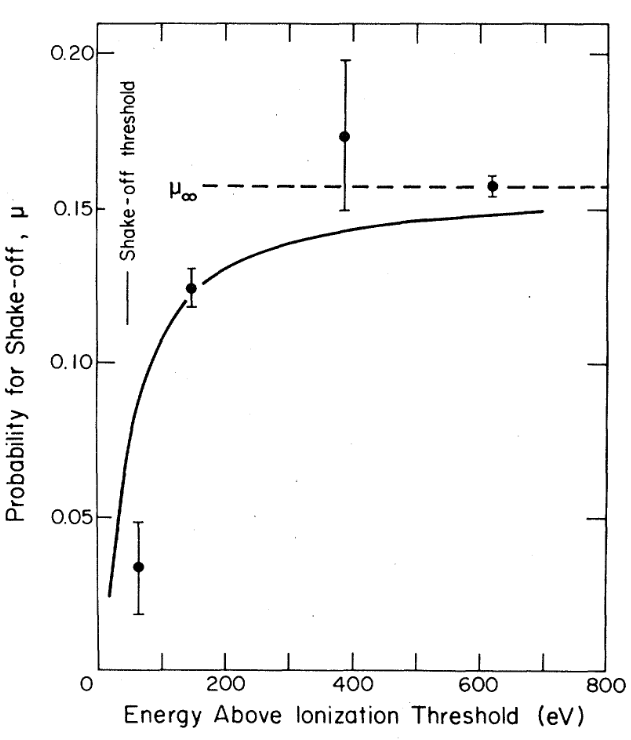
\includegraphics[width=.9\linewidth]{thomas_model.png}
    \caption{Thomas model for shake probability.~\cite{PhysRevLett.52.417}}
    
\end{figure}
    
\end{columns}
\end{frame}


\begin{frame}{Other processes}
    \begin{columns}[T,onlytextwidth]
    \column{0.45\textwidth}
    \begin{block}{Photoexcitation}
        The most relevant process, for the scope of this work, is that of resonant photoexcitation.
        In it, instead of a vacancy generated due to sending one electron to the continuum, it has, in turn, remained bound but in a higher energy level.
    \end{block}
    \column{0.45\textwidth}
        \begin{center}\vspace{-1cm}
    \begin{tikzpicture}[>=stealth',photon/.style={decorate,decoration={snake,post length=1mm}}]
        \draw (0,0) -- (0,1);
        \draw (0,1.2) -- (0,5);
        \draw[-Stealth] (0,5.2) -- (0,6);
        \shade[bottom color=black, top color= white] (0.2,5.3) rectangle (4.2,6);
        
        \draw (-0.1,4.9) -- (0.1,5.1);
        \draw (-0.1,5.1) -- (0.1,5.3);
        \draw (-0.1,0.9) -- (0.1,1.1);
        \draw (-0.1,1.1) -- (0.1,1.3);
        \node[anchor=east,align=center] at (-0.1,0.5) {Inner\\shell};
        \node[anchor=east,align=center] at (-0.1,2.7) {Outer\\shells};
        \node[anchor=east] at (0,6) {$E$};
        
        \draw (0.2,0.5) -- (4.2,0.5);
        \draw (-0.1,0.5) -- (0.1,0.5);
        \draw (.2,2)   --  (4.2,2);
        \draw (.2,2.7)   --  (4.2,2.7);
        \draw(.2,4)  -- (4.2,4);

        
        \draw[fill=SecCol](0.2+4/3,0.5)circle (.2cm);
        \only<1,2>{\draw[fill=SecCol](0.2+8/3,0.5)circle (.2cm)};
        \draw[fill=SecCol](0.2+4/3,2)circle (.2cm);
        \only<1->{\draw[fill=SecCol](0.2+8/3,2)circle (.2cm)};
        \draw[fill=SecCol](0.2+4/3,2.7)circle (.2cm);
        \draw[fill=SecCol](0.2+8/3,2.7)circle (.2cm);

        \draw[fill=SecCol](0.2+8/3,4)circle (.2cm);

        \only<3>{\draw[fill=SecCol,opacity=.3,dashed](0.2+8/3,0.5)circle (.2cm)};




        \only<3>{\draw[fill=SecCol](0.2+4/3,4)circle (.2cm)};
        \only<3>{\draw[-Stealth] (.2+8/3,.7) .. controls (.2+2,1.7)  .. (.2+4/3,3.8)};
        \only<2>{\draw[photon,-Stealth] (4.5,1.5)--(3.,1)};
        
    \end{tikzpicture}
    \end{center}
    \end{columns}
\end{frame}
    
    \subsection{The Hamiltonian}

    \begin{frame}[c]{Schrödinger's Hamiltonian}

    In its most basic form, for a "classical" atom (nucleus + electrons), and when relativistic effects are not taken into account, the considered Hamiltonian follows the one use in Schrödinger's equation:

    \begin{equation*}
        \hat{H}=\displaystyle \sum_i^N\only<1,3->{\frac{1}{2}\laplacian_i}\only<2>{{\color{AlertCol}\frac{1}{2}\laplacian_i}} \only<1-2,4->{- \frac{Z}{r_i}} \only<3>{{\color{AlertCol}- \frac{Z}{r_i}}} + \sum_{j>i}\only<1-3>{ \frac{1}{r_{ij}}}\only<4>{{\color{AlertCol}\frac{1}{r_{ij}}}}
    \end{equation*}
    
    \uncover<2->{It incorporates:
    \begin{itemize}
        \only<1,3->{\item The kinetic energy of the electron.}
        \only<2>{\item {\color{AlertCol}The kinetic energy of the electron.}}
        
        \only<1,2,4>{\item The potential energy of the electron-nucleus attraction.}
        \only<3>{{\color{AlertCol}\item The potential energy of the electron-nucleus attraction.}}
        
        \only<1-3>{\item  The potential energy of the electron-electron repulsion.}
        \only<4>{{\color{AlertCol}\item  The potential energy of the electron-electron repulsion.}}
        
    \end{itemize}}
    \end{frame}

    \begin{frame}[c]{Solving the non-relativistic many-body problem}
        \begin{columns}[T,onlytextwidth]
        \column{0.45\textwidth}
        \only<1-7>{\begin{block}{}
            Due to the complexity introduced by the many bodies in the system, and their interactions, a numerical method needs to be employed as to obtain eigenfunctions for this Hamiltonian.
        \end{block}}
        
        \only<8>{
        \begin{block}{}
            Each of the electrons' wavefunctions, $u$, are composed as a product of a spatial part, $\psi$, and one related to the electron's spin $\chi$.
            \begin{equation*}
                u=\psi \chi
            \end{equation*}
            The system's wavefunction should then be written as a Slater determinant as to account for anti-symetry and the fermionic nature of the electrons.
        \end{block}}
        \only<9>{
        \begin{block}{}
            Through a {\color{AlertCol}self-consistent} field approach, the method solves, for each cycle, a set of integro-differential equations as a way to compute new wavefunctions and the new energy for the system.
        \end{block}
        }
        \only<10>{
        \begin{block}{}
            This process is then repeated up until the energy difference in-between two steps is under a pre-defined benchmark value, as to assure the computation has converged.
        \end{block}
        }

        \column{0.5\textwidth}
        \only<10>{
            METER DIAGRAMA DE BLOCOS
        }
        
        \only<1-7>{
        \begin{center}\vspace{-1cm}
        \begin{tikzpicture}[>=stealth',photon/.style={decorate,decoration={snake,post length=1mm}}]


        \only<3-7>{\draw[photon,->]  (0,0) -- (0,1.2);}
        \only<5-7>{\draw[photon,->]  (0,0) -- (0.707106781*2,0.707106781*2);}
        \only<7>{\draw[photon,->]  (-0.707106781*3,0.707106781*3) -- (0.707106781*2,0.707106781*2);}
        \only<7>{\draw[photon,->]  (-0.707106781*3,0.707106781*3) -- (0,1);}
        \only<5-7>{\draw[photon,->]  (0.707106781*2,0.707106781*2) -- (0,1);}
        \only<7>{\draw[photon,->]  (0,0) -- (-0.707106781*3,0.707106781*3);}

        
        \draw[color=PrimeCol] (0,0) circle (1cm);
        
        \draw[fill=AlertCol,dashed] (0,0) circle (.3cm);
        \only<2->{\draw[fill=SecCol]  (0,1) circle (.2cm);}
        \draw[color=PrimeCol] (0,0) circle (2cm);
        \only<4->{\draw[fill=SecCol]  (0.707106781*2,0.707106781*2) circle (.2cm);}
        \draw[color=PrimeCol] (0,0) circle (3cm);
        \only<6->{\draw[fill=SecCol]  (-0.707106781*3,0.707106781*3) circle (.2cm);}


        \end{tikzpicture}

        \end{center}}
        \only<9>{
        \begin{center}
        \vspace{-1cm}
        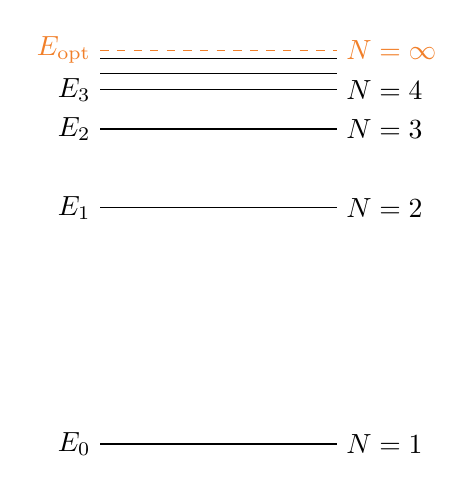
\begin{tikzpicture}
            \node[anchor=east] at (0,0) {$E_0$};
            \node[anchor=east] at (0,3) {$E_1$};
            \node[anchor=east] at (0,4) {$E_2$};
            \node[anchor=east] at (0,4.5) {$E_3$};
            \node[anchor=east,color=AlertCol] at (0,5) {$E_\text{opt}$};

            \node[anchor=west] at (3,0) {$N=1$};
            \node[anchor=west] at (3,3) {$N=2$};
            \node[anchor=west] at (3,4) {$N=3$};
            \node[anchor=west] at (3,4.5) {$N=4$};
            \node[anchor=west,color=AlertCol] at (3,5) {$N=\infty$};
            
            \draw (0,0) -- (3,0);
            \draw (0,3) -- (3,3);
            \draw (0,4) -- (3,4);
            \draw (0,4.5) -- (3,4.5);
            \draw (0,4.7) -- (3,4.7);
            \draw (0,4.9) -- (3,4.9);
            \draw[dashed,color=AlertCol] (0,5) -- (3,5);
        \end{tikzpicture}
            
        \end{center}
        }       

        \only<8>{
        \vspace{1cm}
        \begin{equation*}
            \frac{1}{\sqrt{N!}}\mqty|u_1\qty(x_1)&u_2\qty(x_1)&\hdots&u_N\qty(x_1)\\
                                    u_1\qty(x_2)&u_2\qty(x_2)&\hdots&u_N\qty(x_2)\\
                                    \vdots  &   \vdots  &   \ddots  &   \vdots\\
                                    u_1\qty(x_N)&u_2\qty(x_N)&\hdots&u_N\qty(x_N)|
        \end{equation*}
        }
        \end{columns}
    \end{frame}

    \begin{frame}{Limitations of the non-relativistic approach}

    \begin{columns}[T,onlytextwidth]
    \column{0.45\textwidth}
    While Schrödinger's equation may be quite accurate for low energy systems (e.g. Hydrogen), where the speed of the surrounding electrons is not comparable to that of light, such is not the case for more complex and heavier systems.
    
    \column{0.45\textwidth}
    \begin{block}{Speed of 1s electrons in ground state configurations (\% of $c$)}
        \begin{tabular}{lr}
            Hydrogen:&$0.516\%$\\
            \alert{Copper:}&{\color{AlertCol}$14.751\%$}\\
            Uranium:&$49.211\%$
        \end{tabular}
        \begin{equation*}
            E_k=mc^2\qty(\frac{1}{\sqrt{1-\frac{v^2}{c^2}}}-1)
        \end{equation*}
    \end{block}


    \end{columns}
    \end{frame}

    \begin{frame}{Relativistic approaches}
        \begin{columns}[T,onlytextwidth]
            \column{0.45\textwidth}
            \only<2->{
            \begin{block}{Klein-Gordon equation}
                \begin{itemize}
                    \uncover<3->{\item Incorporates the relativistic energy-mass relation.}
                    \uncover<4->{\item Makes uses of relativistic four-vectors.}
                    \uncover<5->{\item Is Lorentz invariant}
                    \uncover<6->{\item Does not account for the effects of the electron spin (valid for $s=0$).}
                \end{itemize}
            \end{block}}

            \column{0.45\textwidth}
            \only<7->{
            \begin{block}{Dirac equation}
                \begin{itemize}
                    \uncover<8->{\item Includes the same advantages as the previous.}
                    \uncover<9->{\item Accounts for spin interactions.}
                    \uncover<10->{\item Yields two-component solutions, for positive and negative energies.}
                    \uncover<11->{\item The "Dirac sea" originated the talks about the possible existence of anti-particles.}
                \end{itemize}
            \end{block}}
        
            
        \end{columns}        
    \end{frame}

    \begin{frame}{So, what is missing?}
        \only<1,2>{
        \begin{equation*}
                H_D=-\frac{e^2 Z}{r}+\beta m c^2 + \vb{\alpha}\cdot \vb{p}\ c. 
        \end{equation*}}
        \only<3->{\begin{equation*}H= H_D + H_B\end{equation*}}
            \only<2>{\begin{block}{Field retardation effects:}
                Necessary to account for Breit's corrections:
                \begin{equation*}
                    H_B=\sum_{i>j}\frac{e^2}{r_{ij}} - e^2\qty(\frac{\vb*{\alpha}_i\vb*{\alpha}_j}{r_{ij}}+\frac{\qty(\vb*{\alpha}_i \grad_i)\qty(\vb*{\alpha}_j \grad_j)r_{ij}}{2})  ,
                  \end{equation*}
            \end{block}}
            \only<3->{\begin{block}{Field quantization effects (QED):}
                Necessary to account for effects from Quantum Electrodynamics, such as \alert<4>{Self-energy} and \alert<5>{Vacuum Polarization}.

                \begin{center}
                    
                
                \begin{tikzpicture}[remember picture]
                    \only<3>{
                    \begin{feynman}
                        \vertex (a0) at (0,0);
                        \vertex [right=of a0] (a1);
                        \vertex [right= of a1] (a2);
                        \vertex [ right= of a2] (a3);
                        \vertex [ right=of a3] (b1);
                        \vertex [ right=of b1] (b2);
                        \vertex [ right=of b2] (b3);
                        \vertex [ right=of b3] (b4);

                        \diagram*{
                            (a0) --[fermion] (a3),
                            (a1) -- [photon,half left] (a2),
                            

                            (b1) -- [photon] (b2),
                            (b2) -- [fermion,half left] (b3),
                            (b2) -- [anti fermion,half right] (b3),
                            (b3) -- [photon] (b4),
                        };
                    \end{feynman} }    
                    \only<4>{
                    \begin{feynman}
                        \vertex (a0) at (0,0);
                        \vertex [right=of a0] (a1);
                        \vertex [right= of a1] (a2);
                        \vertex [ right= of a2] (a3);
                        \vertex [ right=of a3] (b1);
                        \vertex [ right=of b1] (b2);
                        \vertex [ right=of b2] (b3);
                        \vertex [ right=of b3] (b4);

                        \diagram*{
                            (a0) --[fermion,color=AlertCol] (a3),
                            (a1) -- [photon,half left,color=AlertCol] (a2),
                            

                            (b1) -- [photon] (b2),
                            (b2) -- [fermion,half left] (b3),
                            (b2) -- [anti fermion,half right] (b3),
                            (b3) -- [photon] (b4),
                        };
                    \end{feynman} }    
                    \only<5>{
                    \begin{feynman}
                        \vertex (a0) at (0,0);
                        \vertex [right=of a0] (a1);
                        \vertex [right= of a1] (a2);
                        \vertex [ right= of a2] (a3);
                        \vertex [ right=of a3] (b1);
                        \vertex [ right=of b1] (b2);
                        \vertex [ right=of b2] (b3);
                        \vertex [ right=of b3] (b4);

                        \diagram*{
                            (a0) --[fermion] (a3),
                            (a1) -- [photon,half left] (a2),
                            

                            (b1) -- [photon,color=AlertCol] (b2),
                            (b2) -- [fermion,half left,color=AlertCol] (b3),
                            (b2) -- [anti fermion,half right,color=AlertCol] (b3),
                            (b3) -- [photon,color=AlertCol] (b4),
                        };
                    \end{feynman} }             
                \end{tikzpicture}
            \end{center}
            \end{block}}
    \end{frame}


    
    \subsection{State-of-the-art}

    \begin{frame}{The state-of-the-art}
            \only<1-4>{
            \begin{block}{Reasons for this study}
                \begin{itemize}
                    \item<1-> Copper is a dominant element in today's technological progress.
                    \item<2-> A great deal of studies has been performed on its emission spectrum.
                    \item<3-> Most studies note a skewness in the $K_{\alpha}$ transition lines, being mostly attributed to satellite lines, but leaving open the possibility of its cause coming from \alert{photoexcited states}.
                    \item<4-> Few experiments were performed for the near-threshold region, so theory needs to be formed to accompany new experimental data. 
                \end{itemize}
            \end{block}}
            \only<5->{
                \begin{block}{\textit{mcdfgme} (Multi Configuration Dirac-Fock General Matrix Elements)}
                This code  is a novel computational implementation, based on the Hatree-Fock method, capable of calculating a plethora of atomic parameters, while incorporating all previously mentioned necessary considerations.

                It has proven time and time again to have excellent accuracy and precision when performing calculations for the most varied systems.
            \end{block}}
        
    \end{frame}


    \section{Atomic structure calculations}
    \subsection{The system at study}

    \begin{frame}{The considered excitations}
        As previously stated, the focal point of this work is that of computing radiative relaxation spectra for excited Copper.
        \begin{center}
            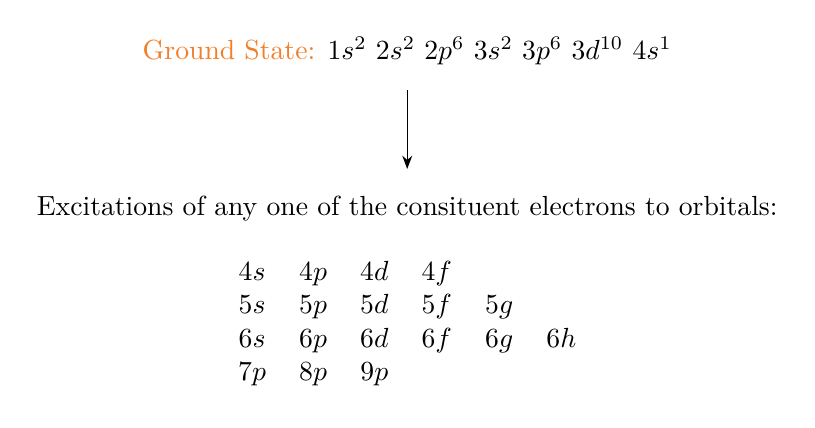
\begin{tikzpicture}[remember picture]
                \node[anchor =center] at (0,0){{\color{AlertCol}Ground State:} $1s^2\ 2s^2\ 2p^6\ 3s^2\ 3p^6\ 3d^{10}\ 4s^{1}$};
                \draw[-Stealth] (0,-0.5) -- (0,-1.5);
                \node[anchor = center] at (0,-2){Excitations of any one of the consituent electrons to orbitals:};
                \node[anchor=north] at (0,-2.5){
                    \begin{tabular}{c c c c c c}
                        $4s$&$4p$&$4d$&$4f$\\
                        $5s$&$5p$&$5d$&$5f$&$5g$\\
                        $6s$&$6p$&$6d$&$6f$&$6g$&$6h$\\
                        $7p$&$8p$&$9p$\\
                       \end{tabular}
                };
             \end{tikzpicture}
        \end{center}

    \end{frame}


    \begin{frame}{The calculated configurations}
        In order to account to all possible decay possibilities, it was necessary to perform calculations for two different sets of configurations.
        \begin{columns}[T,onlytextwidth]
            \column{0.45\textwidth}
            \begin{block}{1-hole configurations}
                Related to the initial and final states of radiative transitions.

                Obtained by running a hole through all orbitals in the base-configurations.
            \end{block}
            \column{0.45\textwidth}
            \begin{block}{2-holes configurations}
                Related to the final states of Auger transitions.

                Obtained by running a combination of two holes through all orbitals in the base-configurations.
            \end{block}
            
        \end{columns}
    \end{frame}

    \subsection{Level calculations}
    

    \begin{frame}{The level manifold}
        \only<1>{It is now necessary to compute all possible levels the studied atomic system can be in. As it will be shown, this is no simple task\dots}

        \only<2->{Besides the original configuration, three other sets of quantum numbers are necessary for defining a level:
        \uncover<3->{
        \begin{itemize}
            \item<3-> The hole orbital labels. $(n\ l_j)$
            \item<4-> The total angular momentum number. $J$
            \item<5-> The eigenvalue/Lagrange multiplier. $\epsilon$
        \end{itemize}}

        }
    \end{frame}

    \begin{frame}{The level manifold- an example: $4p$ excited Copper}
        \begin{columns}[T,onlytextwidth]
            \column{0.55\textwidth}
            \begin{block}{}
            Here, we know two base things:
            \begin{itemize}
                \item The ground state configuration.
                \item One of the electrons was excited to $4p$
            \end{itemize}\end{block}


            \only<3,4>{These are the \alert{labels $(n\ l_j)$}. 7 in total.}

            \only<4>{Let us analyse an excitation from {\color{red} $2p$}.}


            \column{0.4\textwidth}
            \only<2->{
            This leads to the possibility of the electron having come from:
            \begin{itemize}
                \item $1s$
                \item $2s$
                \only<2,3>{\item $2p$}
                \only<4>{\item {\color{red}$2p$}}
                % \item $2p$
                \item $3s$
                \item $3p$
                \item $3d$
                \item $4s$
            \end{itemize}
            }
        \end{columns}
    \end{frame}

    \begin{frame}{The level manifold- an example: $2p\rightarrow 4p$ excited Copper}

        \only<1->{For this configuration, three subshells are open: $2p$, $4s$, and $4p$.}
        
        \only<2->{The different angular momentum couplings lead to various values for \alert{system's total angular momentum}.}

        \only<3->{Possibilities for \alert{$J$} values follow:
        \begin{table}[h!]
            \centering
            \begin{tabular}{cc|cc|cc|c}
                \toprule \multicolumn{2}{c|}{2p}&\multicolumn{2}{c|}{4s}&\multicolumn{2}{c|}{4p}&Total/$J$\\
                $M_l$ & $M_s$ & $M_l$&$M_s$&$M_l$&$M_s$&$M_l+M_s$\\\midrule
                $1$&$-\sfrac{1}{2}$&$0$&$-\sfrac{1}{2}$&$1$&$-\sfrac{1}{2}$&$\sfrac{1}{2}$\\
                $1$&$\sfrac{1}{2}$&$0$&$-\sfrac{1}{2}$&$1$&$-\sfrac{1}{2}$&$\sfrac{3}{2}$\\
                $1$&$\sfrac{1}{2}$&$0$&$\sfrac{1}{2}$&$1$&$-\sfrac{1}{2}$&\only<3>{$\sfrac{5}{2}$}\only<4->{\color{red}{$\sfrac{5}{2}$}}\\
                $1$&$\sfrac{1}{2}$&$0$&$\sfrac{1}{2}$&$1$&$\sfrac{1}{2}$&$\sfrac{7}{2}$\\\bottomrule
            \end{tabular}
        \end{table}
        }
    \end{frame}


    \begin{frame}{The level manifold- an example: $2p\rightarrow 4p$, $J=\sfrac{5}{2}$}

        \only<1>{Even for this \textbf{very} specific example, the branching-out continues:}
        
        \only<2->{There are many possibilities for achieving this certain combination of a given configuration and $J$ value. Each, is represented by the respective \alert{$\epsilon$}.}

        \only<3>{
            \begin{table}[h!]
                \centering
                \begin{tabular}{cc| cc | cc}
                    \toprule\multicolumn{6}{c}{$J=\sfrac{5}{2}$}\\\midrule
                    \multicolumn{2}{c|}{2p}&\multicolumn{2}{c|}{4s}&\multicolumn{2}{c}{4p}\\
                    $M_l$ & $M_s$ & $M_l$&$M_s$&$M_l$&$M_s$\\\midrule
                    $1$&$-\sfrac{1}{2}$&$0$&$\sfrac{1}{2}$&$1$&$\sfrac{1}{2}$\\
                    $1$&$\sfrac{1}{2}$&$0$&$-\sfrac{1}{2}$&$1$&$\sfrac{1}{2}$\\
                    $1$&$\sfrac{1}{2}$&$0$&$\sfrac{1}{2}$&$1$&$-\sfrac{1}{2}$\\\bottomrule
                \end{tabular}
            \end{table}
        }
    \end{frame}


    \begin{frame}{The level manifold}
        This set of possibilities and rearrangements form what we call \alert{the level manifold}. In addition, a $2J+1$ level degeneracy is accounted for.
        \begin{center}
            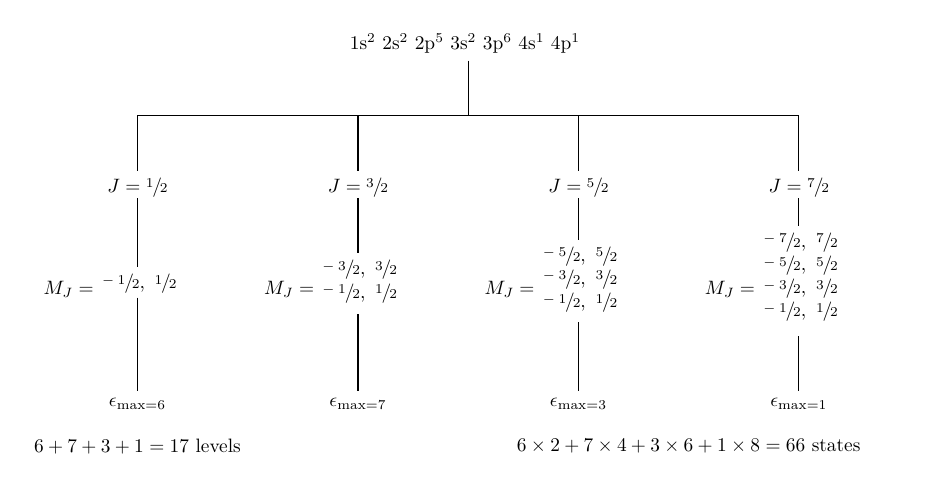
\begin{tikzpicture}[remember picture,scale=.7,transform shape]
                \draw (0,0)node[anchor=south]{$1\text{s}^2\ 2\text{s}^2\  2\text{p}^5\ 3\text{s}^2\ 3\text{p}^6\ 4\text{s}^1\ 4\text{p}^1\ $}--(0,-1);
                \draw (-6,-1) -- (6,-1);
                \draw (-6,-1) -- (-6,-2) node [anchor=north]{$J=\sfrac{1}{2}$};
                \draw (-2,-1) -- (-2,-2)node [anchor=north]{$J=\sfrac{3}{2}$};
                \draw (2,-1) -- (2,-2)node [anchor=north]{$J=\sfrac{5}{2}$};
                \draw (6,-1) -- (6,-2)node [anchor=north]{$J=\sfrac{7}{2}$};
                \draw (6,-2.5) -- (6,-3)node [anchor=north, text centered, align=center, text width=2cm]{
                    $\sfrac{-7}{2},\ \sfrac{7}{2}$
                    
                    $\sfrac{-5}{2},\ \sfrac{5}{2}$
        
                    $\sfrac{-3}{2},\ \sfrac{3}{2}$
        
                    $\sfrac{-1}{2},\ \sfrac{1}{2}$
                    };
                \node at (4.75,-4.15){$M_J =$};
                \draw (2,-2.5) -- (2,-3.25)node [anchor=north, text centered, align=center, text width=2cm]{
                    $\sfrac{-5}{2},\ \sfrac{5}{2}$
                    
                    $\sfrac{-3}{2},\ \sfrac{3}{2}$
        
                    $\sfrac{-1}{2},\ \sfrac{1}{2}$
                    };
                \node at (0.75,-4.15){$M_J =$};
                \draw (-2,-2.5) -- (-2,-3.5)node [anchor=north, text centered, align=center, text width=2cm]{
                    $\sfrac{-3}{2},\ \sfrac{3}{2}$
                    
                    $\sfrac{-1}{2},\ \sfrac{1}{2}$
                    };
                \node at (-3.25,-4.15){$M_J =$};
                \draw (-6,-2.5) -- (-6,-3.75)node [anchor=north, text centered, align=center, text width=2cm]{
                    $\sfrac{-1}{2},\ \sfrac{1}{2}$
                    };
                \node at (-7.25,-4.15){$M_J =$};
                \node[white] at (7.25,-4){$M_J =$};
        
                \node at (-6,-7) {$6+7+3+1= 17$ levels};
                \node at (4,-7) {$6\times 2+7\times 4+3\times6+1\times 8=66$ states};
                \draw (6,-5) -- (6,-6)node[anchor=north]{$\epsilon_{\text{max}=1}$};
                \draw (2,-4.75) -- (2,-6)node[anchor=north]{$\epsilon_{\text{max}=3}$};
                \draw (-6,-4.3) -- (-6,-6)node[anchor=north]{$\epsilon_{\text{max}=6}$};
                \draw (-2,-4.6) -- (-2,-6)node[anchor=north]{$\epsilon_{\text{max}=7}$};
            \end{tikzpicture}
        \end{center}
    \end{frame}

    \begin{frame}{Level calculations with \textit{mcdfgme}}
        A calculation was performed for each existent level.
        
        In each of them, a level was treated as a linear combination of state wavefunctions (associated with the eigenvalues) with mixing coefficients:

        \begin{equation*}
            \ket{\Psi}=a_1\ket{\psi_1}+ a_2\ket{\psi_2} + \dots
        \end{equation*}

        \begin{columns}[T,onlytextwidth]
            \column{0.45\textwidth}
            \begin{block}{Self-consistent field}
                \begin{itemize}
                    \item Coulomb interactions
                    \item Breit considerations
                    \item Vacuum Polarization
                \end{itemize}
            \end{block}
            \column{0.45\textwidth}
            \begin{block}{Perturbation theory}
                Self-energy
            \end{block}
        \end{columns}
    \end{frame}

    \begin{frame}{Evaluating the calculation}
        \begin{columns}[T,onlytextwidth]
           \column{0.45\textwidth}
           \begin{block}{What to look out for:}
            \begin{itemize}
                \item \alert<2>{Orthogonality conservation}
                \item \alert<3>{Energy divergences}
                \item \alert<4>{Effective nuclear charge}
            \end{itemize}
           \end{block}
           \column{.45\textwidth}
           \only<2>{Due to the method's numerical nature, orthogonality problems may surge.

           We look at overlap values for similar orbitals (same $l_j$) and set a maximum threshold:

           \begin{equation*}
            \abs{\braket{n\ l_j}{m\ l_j}}\leq 10^{-6}
           \end{equation*}
           }
           \only<3>{
            A component of the energy is computed through two different methods. For good convergence, the difference in their values should not be above $1\ \si{\electronvolt}$.

            \begin{equation*}
                \abs*{E_1 - E_2}\leq 1\ \si{\electronvolt}
            \end{equation*}
           }
           \only<4>{
            The presence of inner electrons leads to a shielding of the positive nuclear charge. As so, outer electrons will be subject to an attenuated positive charge.

            This effect has been previously studied, and the obtained values should be benchmarked.
           }
        \end{columns}
    \end{frame}

    \begin{frame}{Methods for solving the convergence problems}
        \begin{itemize}
            \item Changing the number of self-consistent cycles.
            \item Altering cycle parameters, such as accuracy.
            \item Choosing the initial trial wavefunctions for select orbitals (e.g. Hydrogenoids or obtained through the Thomas Fermi potential).
            \item Changing the method for solving the Dirac equation.
            \item Enforcing the node number for the wavefunctions
        \end{itemize}
    \end{frame}

    \begin{frame}{Changes in wavefunctions after the variational process}

        \begin{figure}
            \centering
            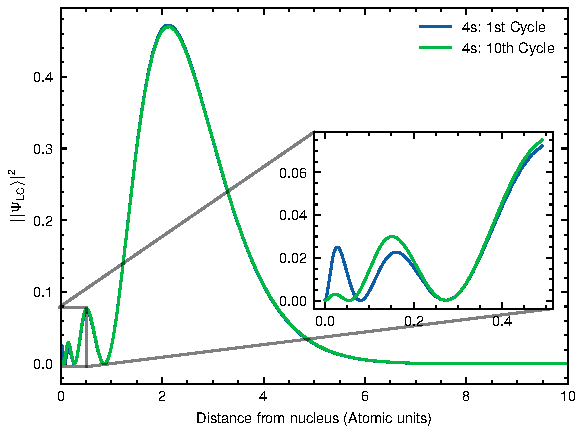
\includegraphics[width=.7\textwidth]{WFcomp.pdf}
        \end{figure}
        
    \end{frame}

    \begin{frame}{Total number of calculated levels}

        \begin{center} For the 19 performed calculations,\end{center}
        \begin{columns}[T,onlytextwidth]
        \column{.45\textwidth}
        \begin{block}{}
            \begin{itemize}
                \item 1601 1-hole levels\begin{itemize}
                    \item 166 manually converged
                \end{itemize}
                \item 20550 2-holes levels\begin{itemize}
                    \item 1678 manually converged
                \end{itemize}
            \end{itemize}
        \end{block}
        \column{.45\textwidth}
        \begin{block}{}
            Leaving a total of:
            \begin{itemize}
                \item 22151 levels calculated
                \item  1844 levels manually converged
            \end{itemize}
        \end{block}
    \end{columns}
    \end{frame}
    
    \subsection{Transition computations}
    \begin{frame}{Atomic transitions}
        When a system is not found in its least energetic state various processes will occur until the most stable one is reached.

        In this way, for every level, calculations were performed for decays to all possible lower energy states.

        \begin{center}
            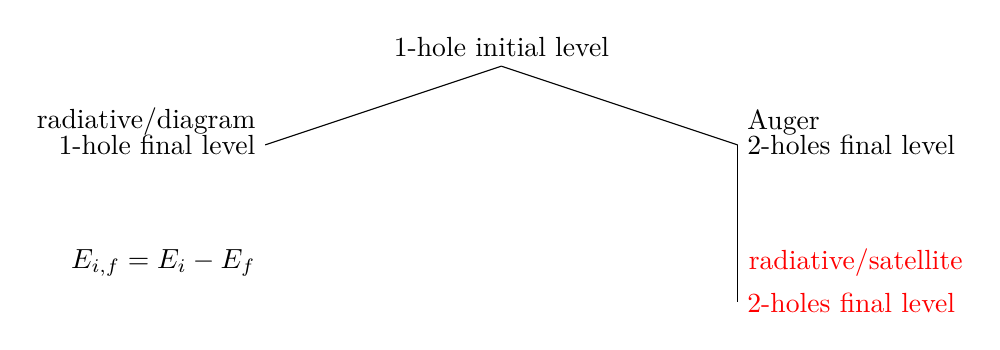
\begin{tikzpicture}[remember picture]
                \node[anchor=south] at (0,0) {1-hole initial level};
                \node[anchor=south east] at (-3,-1) {\alert{radiative/diagram}};
                \node[anchor=south west] at (3,-1) {\alert{Auger}};
                \node[anchor=center] at (4.5,-2.5) {{\color{red}radiative/satellite}};
                \node[anchor=east] at (-3,-1) {1-hole final level};
                \node[anchor=west] at (3,-1) {2-holes final level};
                \node[anchor=west] at (3,-3) {{\color{red}2-holes final level}};
                \draw (0,0) -- (-3,-1);
                \draw (0,0) -- (3,-1);
                \draw (3,-1) -- (3,-3);

                \node[anchor=east] at (-3,-2.5){$E_{i,f}=E_i-E_f$};

            \end{tikzpicture}
        \end{center}
    \end{frame}

    \begin{frame}{Radiative transitions}

        Given the set of all 1-hole levels, with $n$ elements, the total number of these transitions (without accounting for level degeneracy), $N$, is simply given by the amount of combinations of two elements between the set:

        \begin{equation*}
            N=\frac{n!}{2\cdot\qty(n-2)!}
        \end{equation*}

        For these transitions, \alert{full orbital relaxation} was allowed.

        The \textit{mcdfgme} calculation yields the rates for each Electric and/or Magnetic component/pole for both Coulomb (length) and Lorentz (velocity) gauges.
    \end{frame}

    \begin{frame}{Auger transitions}
        The total number of Auger transitions can not be calculated \textit{a priori}. Since the 1-hole and 2-holes level sets are ''independent'', the level structure needs to be calculated in order to fully resolve the number of transitions.



        For computing these transitions, the free-electron wavefunction has to be computed for the initial state potential, and \alert{orthogonality is enforced} between the free-wave and bound orbitals.
    \end{frame}

    \begin{frame}{All calculated transitions}
        In total, for this work,

        \begin{itemize}
            \item<2->70885 diagram radiative
            \item<3->452988 Auger
            \item<4-> 6684258 satellite radiative  
        \end{itemize}
        \only<5->{transitions were calculated, totaling to 7208131 computations performed.}
    \end{frame}

    \begin{frame}{Rate and Energy matrices}
        \only<1>{To evaluate and benchmark a calculation, a visualization tool was used, where the calculated \alert{energy} and \alert{rate} values were displayed in a grid-like view.}
        \only<2>{
            \begin{tikzpicture}[remember picture]
                \node at (0,0){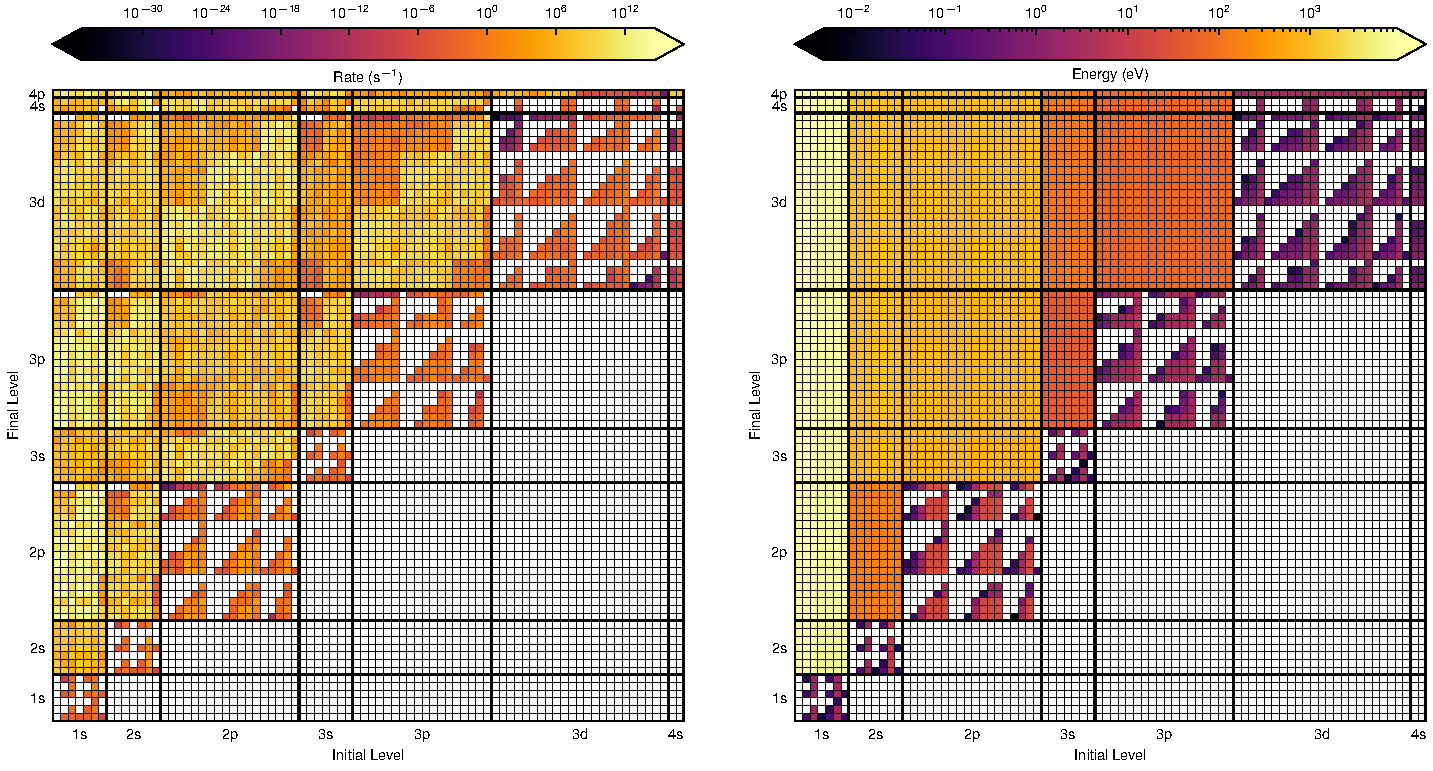
\includegraphics[width=\textwidth]{4p_RM.pdf}};
            \end{tikzpicture}
        }
        \only<3>{
            \begin{tikzpicture}[remember picture]
                \node at (0,0){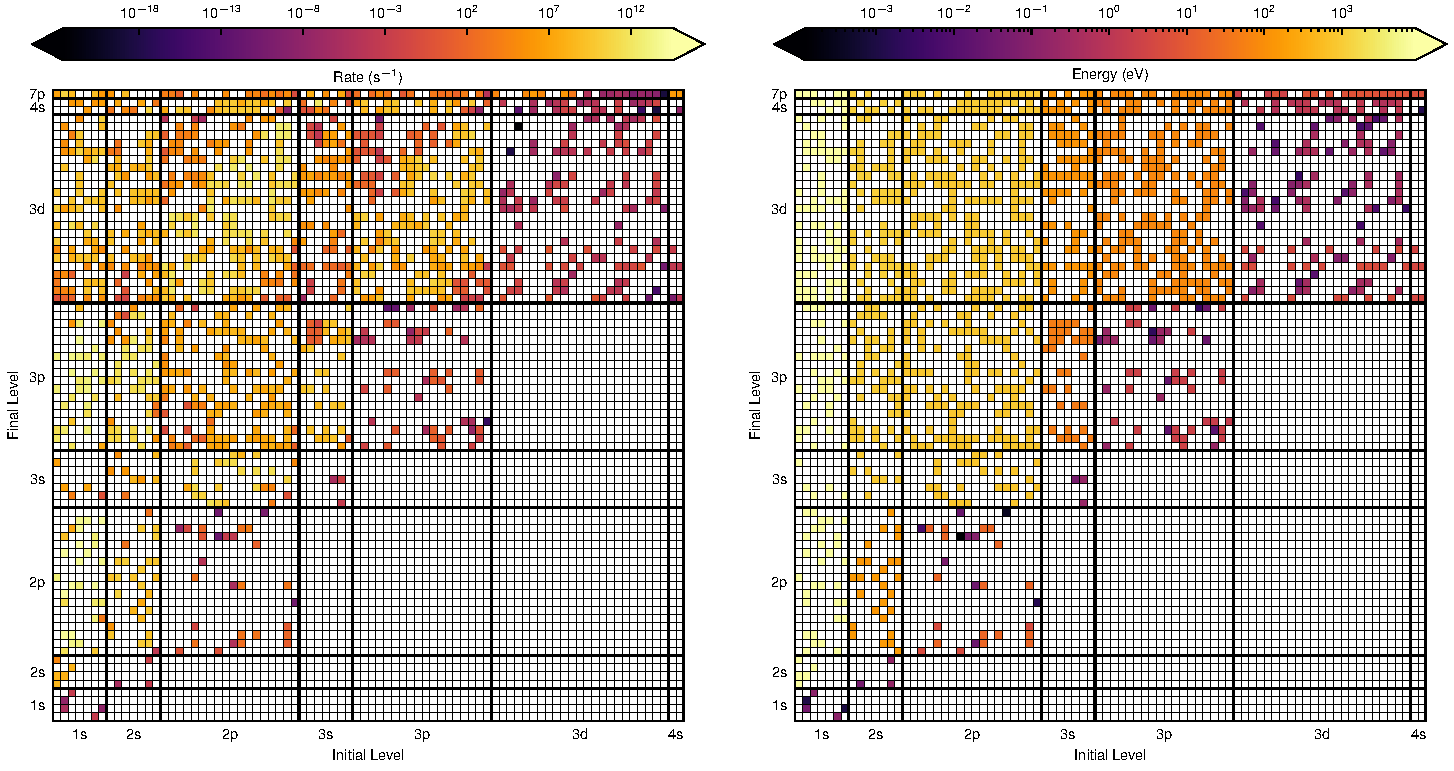
\includegraphics[width=\textwidth]{7p_RM.pdf}};
            \end{tikzpicture}
        }
    \end{frame}

    \subsection{Fundamental atomic parameters}
    \begin{frame}{Total radiative and non-radiative rates}
        \only<1>{After computing all possible transitions, one can now start to evaluate certain atomic parameters.}

        \only<2->{To start, the total radiative and non-radiative rates for each level should be computed. When compared, they can provide information on the probability of said level decaying either way.
        
        
        \begin{equation*}
            R_i^R = \qty(2 J_i + 1 )\sum_f R_{i,f}^R
        \end{equation*}

        \begin{equation*}
            R_i^{NR} = \qty(2 J_i + 1 )\sum_f R_{i,f}^{NR}
        \end{equation*}
        }
    \end{frame}

    \begin{frame}{Fluorescence Yield}
    \only<1>{    The quantity is an indicator of the probability of a level decaying either via the emission of a photon as opposed to an Auger electron.

        It is given by the ratio between the level's radiative and total rates:

        \begin{equation*}
            \omega_i = \frac{R_i^R}{R_i^R+ R_i^{NR}}
        \end{equation*}}

    \only<2>{
            For ionized Copper, the $K$ shell F.Y. was computed to be $45.34\%$.

            \alert{Every calculated excited state presented a value inferior to this.}
            \begin{columns}[T,onlytextwidth]
                \column{.45\textwidth}
                \begin{block}{\centering Minimum value:}
                    \begin{center}
                    {\color{blue}
                    
                    $6s$-excited Copper

                    $18.09\%$}
                \end{center}
                \end{block}
                \column{.45\textwidth}
                \begin{block}{\centering Maximum value:}
                    \begin{center}
                        {\color{red}
                        
                        $4s$-excited Copper
    
                        $44.88\%$}
                    \end{center}
                \end{block}
                
            \end{columns}

            \vspace{.5 cm}
            This decrease can be explained by the \alert{presence of an extra electron} increasing the number of Auger channels.

    }
    \only<3>{
        \begin{block}{Other subshells}
            For other subshells, save for $M_{4,5}$,  the F.Y. slightly oscillated around the obtained value for ionized Copper, but mostly \alert{preserving the same order of magnitude}.
        \end{block}
        \begin{block}{$M_{4,5}$ subshells}
            Curiously both for ionized Copper and for all excitations to $ns$ orbitals, as well as $4p$ and $5p$, \alert{only radiative decays occur}, while for the rest, \alert{Auger transitions reign}.
        \end{block}
    }
    \end{frame}

    \begin{frame}{Level widths}
        \only<1>{Quantum mechanics tells us bound systems are arranged in states with \alert{quantized energy}, hence why a discrete amount of levels was calculated, a not a continuum.}
        \only<2>{It does, however, also alert us to natural uncertainties, as described by the well-known \alert{Heisenberg uncertainty principle}.
        }
        \only<3,4>{While the momentum-position relation is certainly the most famous one, its energy-time counterpart will have implications in the next steps:}
        
        \only<4,5->{\begin{equation*}
            \Delta E \Delta t \geq \hbar
        \end{equation*}
        }

        \only<5->{From this, we can naturally deduce that, a level which decays to other lower energy ones $\qty(R\rightarrow\frac{1}{\Delta t})$, should, in principle, also have an \alert{energy width}.

        As such, we define the level width as:

        \begin{equation*}
            \Gamma_i = \hbar \cdot\qty(R_i^R+R_i^{NR})
        \end{equation*}}

        \only<6>{And the width of a transition as the sum of the widths for the initial and final level:
        \begin{equation*}
            \Gamma_{i,f} = \Gamma_i + \Gamma_f
        \end{equation*}
        }
        
    \end{frame}

    \begin{frame}{Transition intensities}
        Now that many atomic parameters are calculated, it is possible to calculate the spectral intensity of a given transition.

        \begin{equation*}
            I_{i,f} = \alert<4>{N_i}
            \alert<2>{\frac{2J_i+1}{g_{\text{sub}}}}
            \alert<3>{\frac{R_{i,f}}{R_i^R+R_i^{NR}}}
        \end{equation*}

        Put into simple terms, the intensity is nothing more than the product of the statistical weight of the \alert<2>{level multiplicity}, of the \alert<3>{individual rate} compared to the total one, and a \alert<4>{scaling factor accounting for population generation}.
        
    
    \end{frame}

    \section{Spectra simulation}
    \subsection{Line shape}
    \begin{frame}{The theoretical spectral shape}
        \only<1>{Based on all previously computed atomic parameters, it is now possible to start simulating spectral lines.}
        \only<2-4>{
            \vspace{-0.5cm}
            \begin{columns}[onlytextwidth,T]
                \column{.45\textwidth}
                \begin{block}{Lorentzian profile}
                Describes the theoretical line shape for the emission:
                \begin{equation*}
                    \frac{I_{i,f}}{2\pi}\frac{\Gamma_{i,f}}{\qty(E-E_{i,f})^2 + \qty(\Gamma_{i,f}/2)^2}
                \end{equation*}

                Does not account for \alert{thermal distributions} and \alert{stochastic events}.
            \end{block}

            \only<3-4>{
                \column{.45\textwidth}
                \begin{block}{Gaussian profile}
                    This profile will be used to account for any \alert{broadening effects} that may impact the measured spectra.
                    \begin{equation*}
                        \frac{1}{\sigma\sqrt{2\pi}}\exp(-\frac{E^2}{2\sigma^2})
                    \end{equation*}
                \end{block}
            }
            \end{columns}
            \only<4>{\vfill The convolution of both gives rise to the \alert{Voigt profile}, incorporating all the desired effects, at the cost of computational power.}
        }
        \only<5>{
            \begin{figure}
                \centering
                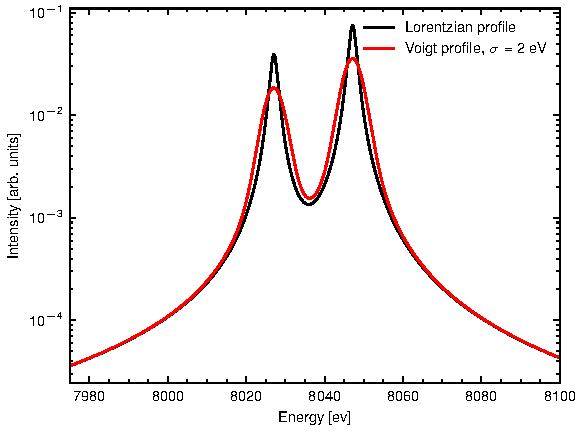
\includegraphics[width=.7\textwidth]{K_lorentz_voigt.pdf}
            \end{figure}
        }
    \end{frame}

    \begin{frame}{The incident beam}
        For the purpose of this work, the desired source of radiation for such study would be a synchrotron line.

        \begin{itemize}
            \item Due to the usage of wigglers and undulators, the beam can be close to monochromatic.
            \item The energy of the radiation used is tunable, allowing for the survey from regions below to post-ionization threshold.
        \end{itemize}

        As such, a beam profile of $0.5\ \si{\electronvolt}$ was considered.
    \end{frame}

    \subsection{Photoexcitation}
    \begin{frame}{What about $N_i$? The photoexcitation effect}
       \only<1>{The computation of this parameter is somewhat tricky.
        \begin{itemize}
            \item No analytical expression for cross-sections could be found.
            \item Should be calculated ab-initio (no data from outside).
            \item Must simulate the resonance effect.
            \item Needs to be valid (according to the laws of physics).
            \item The beam profile should be considered.
        \end{itemize}}
        \only<2>{\framesubtitle{The proposed solution:}
        To solve this problem, an \textit{ad-hoc} expression was developed.

        The \alert{rate} and \alert{energy} of the transition from ground state to the excited state was considered by looking at the inverse transition.
        \begin{center}
            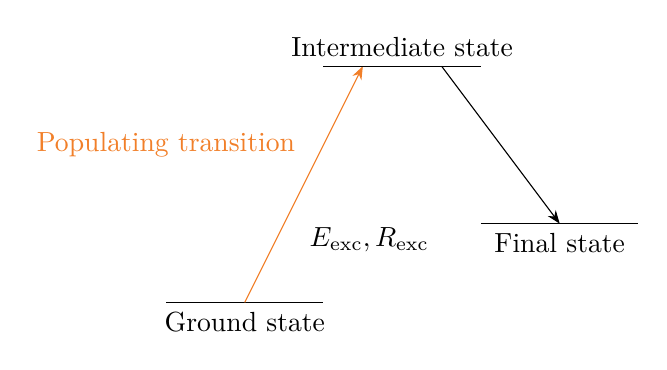
\begin{tikzpicture}[remember picture]
                \draw (0,0) -- (2,0);
                \node[anchor=north] at (1,0) {Ground state};
                \draw[-Stealth,AlertCol] (1,0) -- (2.5,3);

                \draw (2,3) -- (4,3);
                \node[anchor=south] at (3,3) {Intermediate state};

                \draw (4,1) -- (6,1);
                \node[anchor=north] at (5,1) {Final state};
                \draw[-Stealth] (3.5,3) -- (5,1);

                \node at (0,2){{\color{AlertCol}Populating transition}};
                \node[anchor=west] at (1.7,0.8){\alert{$E_{\text{exc}},R_{\text{exc}}$}};
            \end{tikzpicture}
        \end{center}
        }

        \only<3>{
        A Lorentzian profile was then created using both the energy value, and the associated  rate. The overlap between this profile and the beam's was computed and multiplied by the rate:

        \begin{equation*}
            N_i=R_{\text{exc}}\int_{-\infty}^{\infty} G\qty(E-E_{\text{beam}},0.5\ \si{\electronvolt})\cdot L\qty(E-E_{\text{exc}},\Gamma_{\text{exc}})\ \dd{E}
        \end{equation*}

        }
    \end{frame}

    \begin{frame}[plain]
        \begin{figure}
            \centering
            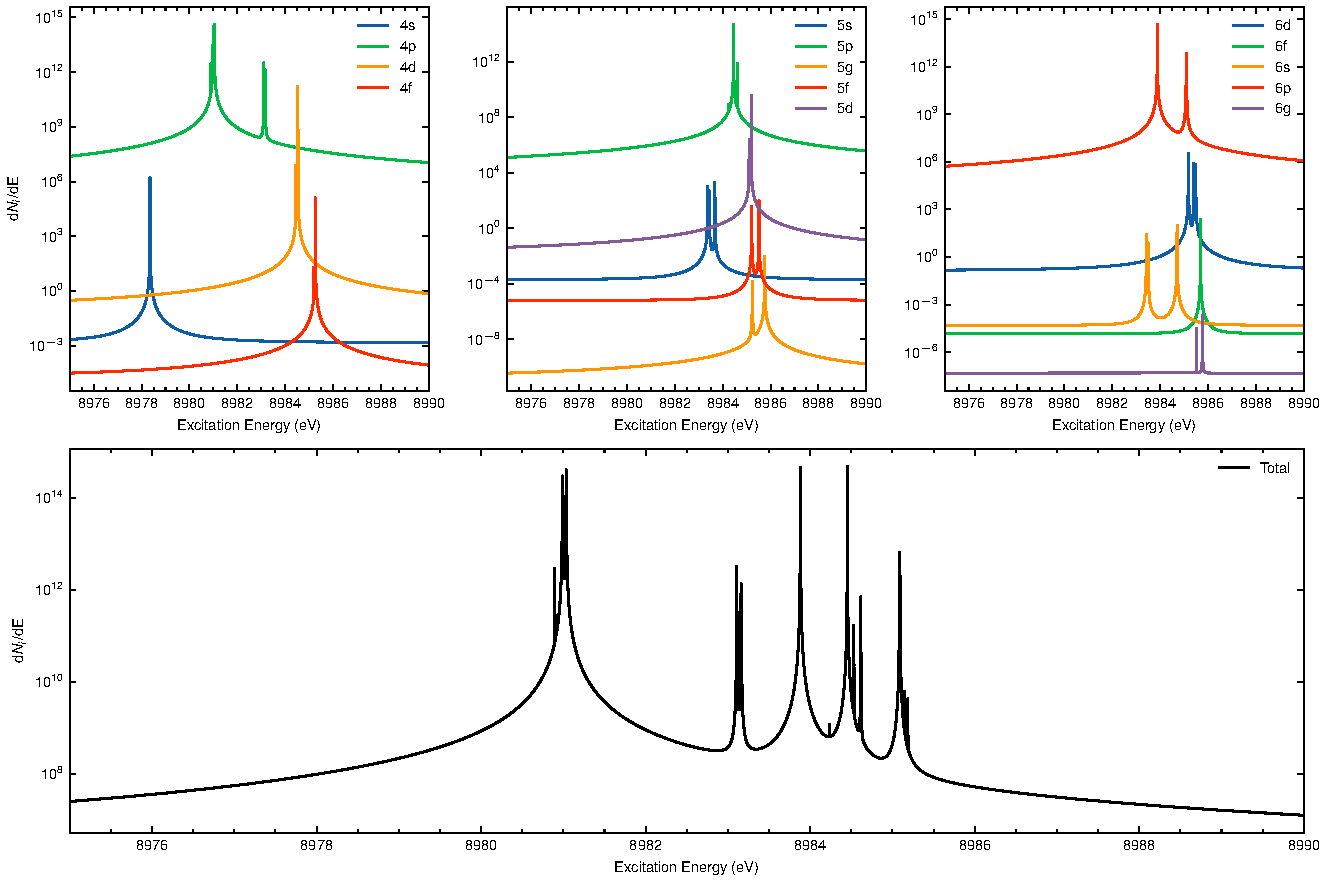
\includegraphics[width=\textwidth]{absorption.pdf}
        \end{figure}
    \end{frame}



    
    \subsection{Photoionization}

    \begin{frame}{What about $N_i$? The photoionization effect}
        \only<1>{
        For energies over the threshold, ionization starts to occur. This effect, will be the predominant one, once the threshold is reached.

        For K-shell ionization, there are \alert{two possible levels}, with different values of total angular momentum:

        \begin{columns}[onlytextwidth,T]
            \column{.45\textwidth}
            \begin{block}{\centering$J=0$}
                \begin{itemize}
                    \item $1s$, $4s$ counteraligned spins.
                    \item Multiplicity of 1
                    \item Edge energy of $8986.02\ \si{\electronvolt}$
                \end{itemize}
            \end{block}
            \column{.45\textwidth}
            \begin{block}{\centering$J=1$}
                \begin{itemize}
                    \item $1s$, $4s$ aligned spins.
                    \item Multiplicity of 3
                    \item Edge energy of $8985.93\ \si{\electronvolt}$
                \end{itemize}
            \end{block}
        \end{columns}}

        \only<2>{

        The differential oscillator strength were calculated by performing \textit{mcdfgme} calculations for different incoming photon energies:

        \begin{columns}[onlytextwidth,c]
            \column{.5\textwidth}
            \begin{figure}
                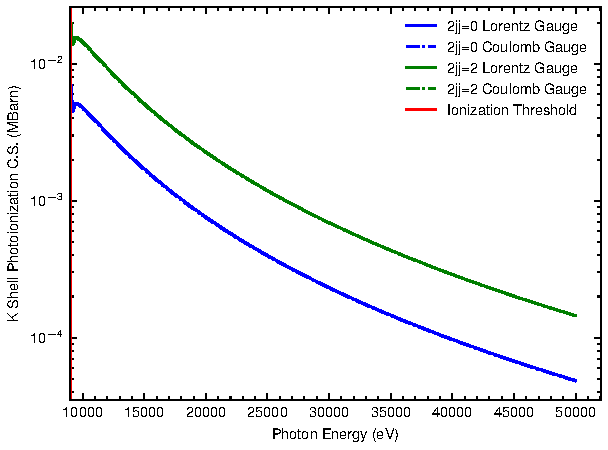
\includegraphics[width=\textwidth]{both_50keV.pdf}
            \end{figure}

            \column{.47\textwidth}
            \begin{block}{Oscillator strength $\leftrightarrow$ Rate}
                \begin{equation*}
                    O_s=2.304\cdot 10^{-8}\qty[\si{\electronvolt^2\second}]\cdot\frac{g_{fin}/g_{in}}{E^2}\cdot R
                \end{equation*}
            \end{block}
        \end{columns}
        }
        \only<3>{In a similar fashion, $N_i$ was computed by the overlap between these profiles  and the beam's.}
    \end{frame}

    \subsection{The synthetic spectrum}

    \begin{frame}{Compiling the results}
        \only<1>{After this extremely extensive process, it is now finally possible to account for every interaction, and build a synthetic spectrum.} \only<2>{By accounting for every one of the thousands of computed transitions we get\dots}
    \end{frame}

    \begin{frame}{The final spectrum}
        {\color{red}MUDAR A IMAGEM PARA MAIS RECENTE}
        \begin{figure}
            \centering
            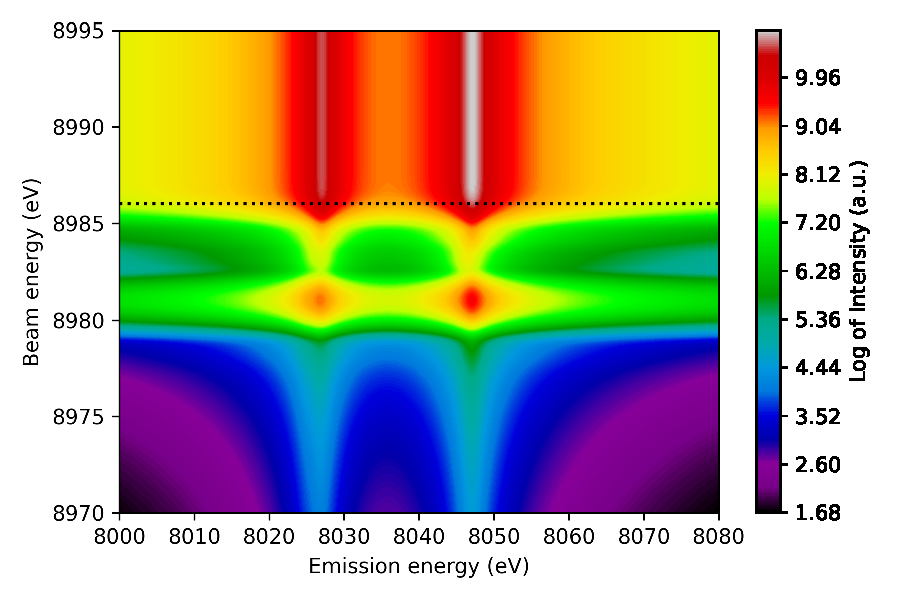
\includegraphics[width=.8\textwidth]{all_log_alt.pdf}
        \end{figure}
    \end{frame}

    \section{Spectral Analysis}

    \begin{frame}{The analysis profiles}

        \only<1>{As previously stated, each spectral line is, in reality composed by a great set of many others. As such, it is not expected to be symmetric, and single Lorentzian and Gaussian profiles are not suited for spectral analysis.}
        \only<2->{For each spectral line ($K_{\alpha_1}$ or $K_{\alpha_2}$), an asymmetric Lorentzian profile was fitted, and an analysis was performed throughout the beam energies.
        
        \begin{equation*}
            \frac{\alert<4>{I}}{2\pi}\frac{\alert<6>{\Gamma}}{\qty(\frac{E-\alert<5>{E_x}}{\alert<7>{\alpha}\cdot \text{sign}\qty(E-\alert<5>{E_x})+1})^2+\qty(\alert<6>{\Gamma}/2)^2}
        \end{equation*}
        }

        \only<3->{Aside from the \alert<4>{Intensity}, the \alert<5>{Energy}, and the \alert<6>{Width} parameters, it also now includes an \alert<7>{asymmetry index}.}
    \end{frame}
    \subsection{The theoretical results}

    \begin{frame}{Transition energy}
        
    \end{frame}

    
    \begin{frame}{Transition width}
        
    \end{frame}

    
    \begin{frame}{Spectral intensity}
        
    \end{frame}

    
    \begin{frame}{Asymmetry index}
        
    \end{frame}

    \subsection{Comparison with experimental data}

    \begin{frame}{Experimental spectrum from a synchrotron line}
        
    \end{frame}
    \section{A new parallelization code}
    \subsection{The MPI approach}
    
    \begin{frame}{Why the necessity?}
        \only<1>{As previously stated, the amount of calculations needed to be performed makes manual calculations simply unfeasible.}

        \only<2>{   {\color{red} But is a simple automation algorithm enough?}


        No, even with a conventional implementation of an automation script, the amount of time to needed for the computation would still be unreasonable.
        }

        \only<3>{

        {\color{red} The solution? Parallelization.}

        A \textit{master-rank} implementation was used in order to tackle this challenge.
        \begin{itemize}
            \item Using Python due to its flexibility
            \item Using MPI due to its scalability
            \item Able to exploit the computer's physical threads.
        \end{itemize}
            \begin{center}
                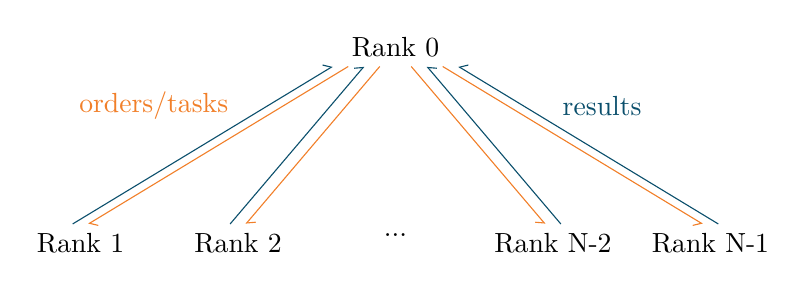
\begin{tikzpicture}[remember picture]


                    \node[anchor=south] at (0,0) {Rank 0};

                    \node[anchor=north] at (-4,-2) {Rank 1};
                    \node[anchor=north] at (-2,-2) {Rank 2};
                    \node[anchor=north] at (0,-2) {...};
                    \node[anchor=north] at (4,-2) {Rank N-1};
                    \node[anchor=north] at (2,-2) {Rank N-2};

                    \draw [-{Straight Barb[left]},AlertCol] (0-0.6,0) -- (-4
                    +.1,-2);
                    \draw [-{Straight Barb[left]},PrimeCol] (-4-0.1,-2) -- (0-0.8,0);
                    
                    \draw [-{Straight Barb[left]},AlertCol] (0-0.2,0) -- (-2
                    +.1,-2);
                    \draw [-{Straight Barb[left]},PrimeCol] (-2-0.1,-2) -- (0-0.4,0);


                    \draw [-{Straight Barb[right]},AlertCol] (0+0.6,0) -- (+4
                    -.1,-2);
                    \draw [-{Straight Barb[right]},PrimeCol] (4+0.1,-2) -- (0+0.8,0);
                    
                    \draw [-{Straight Barb[right]},AlertCol] (0+0.2,0) -- (2
                    -.1,-2);
                    \draw [-{Straight Barb[right]},PrimeCol] (2+0.1,-2) -- (0+0.4,0);
                    \node[anchor=east,color=AlertCol] at (-2,-0.5) {orders/tasks};
                    \node[anchor=west,color=PrimeCol] at (2,-0.5) {results};

                \end{tikzpicture}
            \end{center}
            
        }      


    \end{frame}


    
    \subsection{Speedup comparison}
    
    \begin{frame}{Comparison with other implementations}

        \begin{figure}
            \centering
            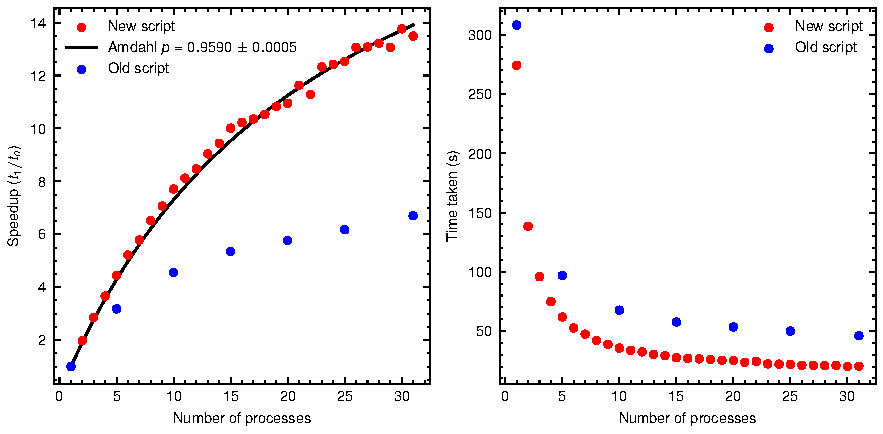
\includegraphics[width=\textwidth]{amdahl.pdf}
        \end{figure}

    \end{frame}

    \miniframesoff
    \appendix
    \section*{+}
 \begin{frame}{Conclusion}
     
 \end{frame}

 \begin{frame}[plain]{}
 \begin{center}
     \Huge Thank you\\
     for your attention!
 \end{center}

 
      \begin{tikzpicture}[remember picture,overlay]
      
         \begin{feynman}
             \vertex (a0) at ([yshift=1.5cm,xshift=-3cm]current page.south);
             \vertex[right=1cm of a0] (a1);
             \vertex[right=1cm of a1] (a2);
             \vertex[above=1.5cm of a2] (a3);
             \vertex[right=2cm of a3] (a4);
             \vertex[right=3cm of a2] (a5);
             \vertex[right=1cm of a5] (a6);
             \vertex[above=.5cm of a3] (v1);
             \vertex[right=.15cm of v1] (v2);
             \vertex[left=.15cm of a4] (v3);
             \vertex[below=.5cm of v3] (v4);
             \vertex[below=.16667cm of v2] (b1);
             \vertex[right=.28cm of b1] (b2);
             \vertex[right=.28cm of b2] (b3);
             \vertex[below=.16667cm of b3] (b4);
             \vertex[above=.16667cm of v4] (c1);
             \vertex[left=.28cm of c1] (c2);
             \vertex[above=.16667cm of c2] (c3);
             \vertex[left=.28cm of c3] (c4);
             \vertex[left=.1cm of v2] (m1);
             \vertex[below=.2cm of m1] (m2);
             \vertex[left=.23cm of v4](m3);
             \vertex[below=.2cm of m3](m4);
             \diagram*{
             % (a0) -- (a2),
             (a1) --[photon,quarter left](a3),
             (a3) --[half left](a4),
             (a3) --[half right](a4),
             (a0) --[fermion] (a6),
             (a4) --[photon,quarter left](a5),
             % (a5) -- (a6),
             (v2) --[photon] (b2),
             (c4) --[photon] (b4),
             (v4) --[photon] (c2),
             % (b3) -- (b4)
             (b2) -- [half left] (b4);
             (b2) -- [half right] (b4);
             (c2) -- [half left] (c4);
             (c2) -- [half right] (c4);
             (m4) --[photon,quarter left] (m2);
             };
             
         \end{feynman}
     \end{tikzpicture}
     
 \end{frame}


\end{document}